\section{Adiabatic Factorization Algorithm}

To end, we introduce the adiabatic factorization protocol. In this section, we make clear that it is different from the gate-based version. To finish this section, we can already mention many-body terms that appear in the adiabatic factorization method. To this section, we can use the discussions done during the meetings, and the papers you used to learn about it.

{\color{red}Here I include a discussion to help you to understand our goals and advances... Also, you can use it in your thesis and get inspired to explain the adiabatic theorem...}

An adiabatic algorithm works as follow. Following the standard strategy of adiabatic algorithms, the solution of the problem is encoded in the problem Hamiltonian $\hat{H}_{\mathrm{P}}$, and then we define a time-dependent adiabatic Hamiltonian $\hat{H}_{\mathrm{ad}}(t)$ such that the initial state of the system is eigenstate of $\hat{H}_{\mathrm{ad}}(t)$ at the time $t=0$ associated to the $n$-th eigenstate $\ket{E_{n}(0)}$ energy level with initial energy $E_{n}(0)$. So, as depicted in Fig.~XX, if the evolution is done through an adiabatic evolution (very slowly-varying $\hat{H}_{\mathrm{ad}}(t)$), at the end of the dynamics, say $t=\tau$, the state of the system will be $\ket{E_{n}(\tau)}$ which is the \textit{update} $n$-th eigenstate of adiabatic Hamiltonian at the instant of time $t = \tau$. In particular, as shown in Fig.~XX, adiabatic algorithms evolves from initial ground states because those states are protected against some kinds of decoherence, and undesired transitions can be suppressed by properly protecting couplings between the ground and first excited states. However, according to the adiabatic theorem, notice that $\ket{E_{n}(0)}$ does not be the fundamental state of $\hat{H}_{\mathrm{ad}}(0)$, and we could start the evolution from an arbitrary state as shown in Fig.~XX. In this case, the transitions like $\ket{E_{n}(t)}\rightarrow\ket{E_{n-1}(t)}$ or $\ket{E_{n}(t)}\rightarrow\ket{E_{n+1}(t)}$ have to be avoided by properly driving the system according to the conditions to adiabaticity. The main problem is that, in those case, the ground-state protection is no longer valid because we started evolutions from states with higher energies. However, in absence of any undesired external effect, the algorithm works perfectly according adiabatic theorem and its validity conditions.

Therefore, if we know that the solution of a given problem is encoded in the $n$-th eigenstate of $\hat{H}_{\mathrm{P}}$, we just need to choose $\hat{H}_{\mathrm{ad}}(t = \tau) = \hat{H}_{\mathrm{P}}$. This can be done, for example, using the following time-dependent Hamiltonian
\begin{equation}
	\hat{H}_{\mathrm{ad}}(t) = \left(\frac{t}{\tau}\right) \hat{H}_{\mathrm{I}} + \left(1 - \frac{t}{\tau}\right) \hat{H}_{\mathrm{P}} 
\end{equation}
where $\hat{H}_{\mathrm{I}}$ is the initial Hamiltonian we can define in the way we want to. For example, in case we start the system of $N$ qubits in a superposition of the form $\ket{\psi(0)} = \ket{+}_{1}\ket{+}_{2}\ket{+}_{3}\cdots \ket{+}_{N}$, here $\ket{+}$ is the eigenstate of the Pauli matrix $\hat{\sigma}^{x}$, we can choose an initial Hamiltonian of the form $\hat{H}_{\mathrm{I}} = \sum_{n=1}^{N} \hat{\sigma}^{x}_{n}$, or $\hat{H}_{\mathrm{I}} = \sum_{n=1}^{N} \hat{\sigma}^{z}_{n}$. This is a free choice and it depends on the way you encode the solution of the problem in the Hamiltonian $\hat{H}_{\mathrm{P}}$. 

\begin{figure}[t!]
	\includegraphics[width=\linewidth]{figs/drawing.pdf}
	\caption{Put your caption here. Put your caption here. Put your caption here. Put your caption here. Put your caption here. Put your caption here. Put your caption here. Put your caption here. Put your caption here. Put your caption here. Put your caption here. Put your caption here.}
	\label{Fig:label}
\end{figure}

Then, to discuss our factorization approach, we can state that we use the binary encoding. To encode a state we use the binary encoding of a natural number. To this end, we use that any natural number $n$ can be written as $n=\sum_{j=0}^{N_\mathrm{bits}-1} x_j \cdot 2^{j}$, for a bit-string values $\textbf{x} = x_{N_\mathrm{bits}-1} x_{N_\mathrm{bits}-2}  \cdots x_{0}$, where each $x_j$ is a dichotomic defined as $x_n \in \{0,1\}$. Using this way to encode natural numbers, we can then introduce the adiabatic algorithm for factorization.

As explained in Ref.~XX, the algorithm is used to solve the following equation
\begin{equation}
	f(p,q) = (N - p \cdot q)^2 = 0 \label{Eq:Quadratic}
\end{equation}
with $p$ and $q$ the two number that factorizes $N$. To simplify the algorithm even more, we use the fact that $p$ and $q$ can be written as $p = 2p^\prime + 1$ and $q = 2q^\prime + 1$, where we can encode the information of $p^\prime$ and $q^\prime$ using $n_p$ and $n_q$ qubits, respectively. In this way, the total number of qubits required is $n = n_p +n_q$. For simplicity, we consider the qubits placed as
\begin{equation}
	\ket{\Psi} = \underbrace{\ket{\psi_{1}}\otimes \cdots \otimes \ket*{\psi_{n_p}}}_{\ket*{\Psi_{p^\prime}}} \underbrace{\ket*{\psi_{n_p+1}}\otimes \cdots \otimes \ket*{\psi_{n_p +n_q}}}_{\ket*{\Psi_{q^\prime}}},
\end{equation}
such that an arbitrary state of the system reads as
\begin{equation}
	\ket{\Psi} = \ket*{\Psi_{p^\prime}} \otimes \ket*{\Psi_{q^\prime}} ,
\end{equation}
and the information about $p^\prime$ and $q^\prime$ are encoded in $\ket*{\Psi_{p^\prime}}$ and $\ket*{\Psi_{q^\prime}}$, respectively. In this way, defining the Pauli matrices such that $\hat{\sigma}^{z}\ket{x} = (-1)^{x}\ket{x}$, we can encode the solution of Eq.~\eqref{Eq:Quadratic} in the ground state of the quadratic problem Hamiltonian~\cite{PhysRevA.104.L050403}
\begin{equation}
	\hat{H}_{\mathrm{QP}} = \left[ N\1 - \left(\sum_{\ell=1}^{n_p} 2^{\ell} \hat{x}_{\ell} + \1 \right)\left(\sum_{m=1}^{n_q} 2^{m} \hat{y}_{m} + \1 \right)\right]^2
\end{equation}
where $\hat{x}_{\ell} = (\1 - \hat{\sigma}_{\ell}^{z})/2$ and $\hat{y}_{m} = (\1 - \hat{\sigma}_{m}^{z})/2$. As for the initial Hamiltonian, in this case, the adiabatic algorithm required the initial state is $\ket{\psi(0)} = \ket{+}_{1}\ket{+}_{2}\ket{+}_{3}\cdots \ket{+}_{N}$, here $\ket{+}$, because we need to give as input all possible solutions of the problem. In this case, we can choose an initial Hamiltonian of the form $\hat{H}_{\mathrm{I}} = -\sum_{n=1}^{N} \hat{\sigma}^{x}_{n}$, where the ``$-$" sign has to be included to make sure $\ket{\psi(0)}$ is ground state of $\hat{H}_{\mathrm{I}}$. So, following the adiabatic theorem, by starting the system in the ground sate a initial Hamiltonian $\hat{H}_{\mathrm{I}}$, and if the evolution is sufficiently slow, the system will be driven through an adiabatic trajectory in which the ground state of $\hat{H}_{\mathrm{QP}}$ is the final state of the system. Therefore, the final state encodes the solution of the problem. 

{\color{red}Maybe, again, mention the problems related to $\hat{H}_{\mathrm{QP}}$... $\hat{\sigma}_{\ell}^{z} \hat{\sigma}_{m}^{z} \hat{\sigma}_{k}^{z}$ and $\hat{\sigma}_{\ell}^{z} \hat{\sigma}_{m}^{z} \hat{\sigma}_{k}^{z}\hat{\sigma}_{n}^{z}$ terms...} In order to solve this challenge, we introduce here the linearized version of $\hat{H}_{\mathrm{QP}}$ using the adiabatic theorem to support our solution.

As a first remark, notice that the Hamiltonian $\hat{H}_{\mathrm{QP}}$ is engineered in order to encode the solution of the problem in its ground state, where the power $2$ is used to get an optimal solution around the value $x$ around $q\cdot p$, as depicted in Fig.~XX. This is why people use the expected value of the energy of $\hat{H}_{\mathrm{QP}}$ in QAOA algorithms. But, as we know, it is not mandatory, and we can simplify the problem as follow. 

\begin{figure}[t!]
	\centering
	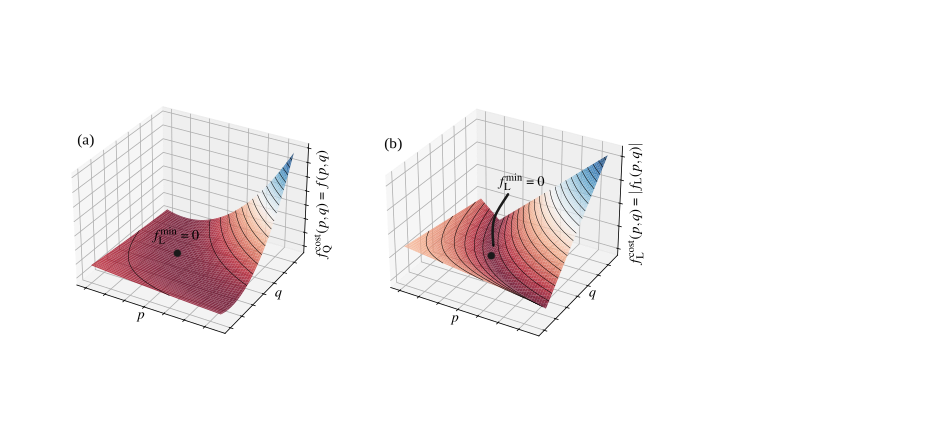
\includegraphics[width=0.9\linewidth]{figs/grafico_3d.pdf}
	\caption{Put your caption here. Put your caption here. Put your caption here. Put your caption here. Put your caption here. Put your caption here. Put your caption here. Put your caption here. Put your caption here. Put your caption here. Put your caption here. Put your caption here.}
	\label{Fig:Graph3D}
\end{figure}

The adiabatic theorem does not impose that the evolution has to start in the ground state of $\hat{H}_{0}$. In principle, by starting in the $n$-th eigenstate $\ket{E_{n}(0)}$ of $\hat{H}_{0}$, the system undergoes an adiabatic evolution with all population in the updated $n$-th state $\ket{E_{n}(t)}$, up to a global phase. Therefore, the adiabatic theorem does not forbid an adiabatic algorithm to work in case the solution is encoded in an eigenstate other than the ground state. Based on this result, we stablish the hypothesis that we can engineer a linearized problem Hamiltonian for factorization $\hat{H}_{\mathrm{LP}}$.

The Hamiltonian $\hat{H}_{\mathrm{LP}}$ is defined through the same logic used to obtain $\hat{H}_{\mathrm{QP}}$, which allows us to define
\begin{equation}
	\hat{H}_{\mathrm{LP}} = N\1 - \left(\sum_{\ell=1}^{n_p} 2^{\ell} \hat{x}_{\ell} + \1 \right)\left(\sum_{m=1}^{n_q} 2^{m} \hat{y}_{m} + \1 \right) ,
\end{equation}
where the desired solution is not the ground state of $\hat{H}_{\mathrm{LP}}$, but it is the eigenstate of $\hat{H}_{\mathrm{LP}}$ with zero eigenstate. Therefore, we have to search for solutions of $\ket{\psi_{\mathrm{out}}}$ such that $\bra{\psi_{\mathrm{out}}}\hat{H}_{\mathrm{LP}}\ket{\psi_{\mathrm{out}}} = 0$, which is similar to search for the zero's solution of the cost function $f_{\mathrm{L}}(p,q) = N - p \cdot q$. The problem here is that any optimization algorithms applied to this problem will provide solutions which minimizes $f_{\mathrm{L}}(p,q)$, and the minimum value of $f_{\mathrm{L}}(p,q)$ does not satisfy $f_{\mathrm{L}}^{\mathrm{min}} = 0$. 

To bypass this problem, we exploit the freedom over the cost function $f^{\mathrm{cost}}_{\mathrm{L}}(p,q)$ defined for QAOA implementations. In fact, while the QAOA problem Hamiltonian is defined as , the cost function is defined as $f^{\mathrm{cost}}_{\mathrm{L}}(p,q) = |f_{\mathrm{L}}(p,q)|$, and therefore the output state will be driven to a solution such that minimizes $f^{\mathrm{cost}}_{\mathrm{L}}(p,q)$, that is, the solution of $|f_{\mathrm{L}}(p,q)|=0$ that is the same solution as $f_{\mathrm{L}}(p,q)=0$. In summary, as shown in Fig.~XX, both $f^{\mathrm{cost}}_{\mathrm{L}}(p,q)$ and $f(p,q)$ have the same minimum around $p \cdot q = N$, and we can use this as input of our QAOA algorithm.

